\clearpage
\section{手持医疗包的绘制}

玩家按下 H，机器人从腰侧取出医疗包，把它贴到胸前，再收回腰侧。货场里的围栏、路面和发电机都留在原处。旧版在手臂移动时重新读取了整座货场的模型，建立供光线查询的三角形索引。画面于是停住一两秒，恢复时手已经到了下一个位置。

\begin{center}
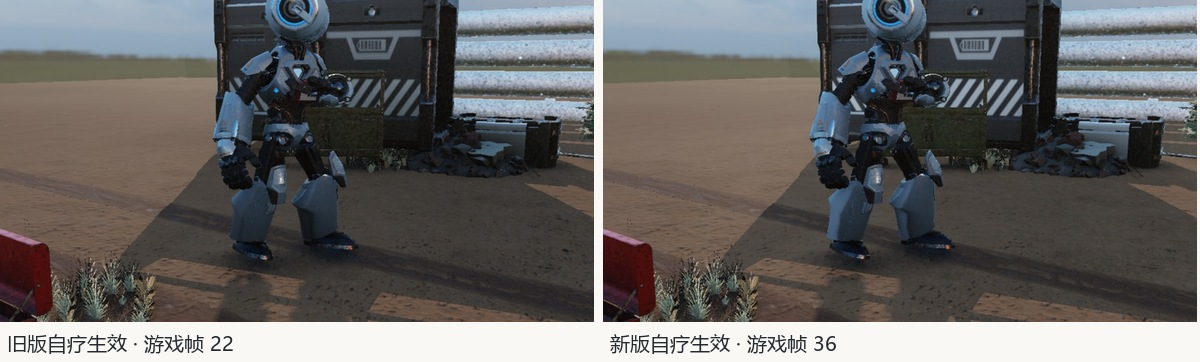
\includegraphics[width=.87\linewidth]{../../../output/validation/packaged-watt/hand-actions/performance/hand-at-contact.jpg}
\end{center}
图中两次自疗使用同一个关卡副本、机位和 H 键输入。两幅取自生命值由 40 增至 90 时的实际窗口。两个时刻的姿势略有差别，连续性要看中间究竟画出了几帧。

\begin{center}
{\smalltable\begin{tabularx}{.95\linewidth}{@{}Xrrrr@{}}\toprule
发行程序 / 次序 & 动作帧数 & 整帧中位 (ms) & 最长帧 (ms) & 重建次数\\\midrule
旧版，第 1 次 & 5 & 1811.0 & 1877.9 & 4\\
新版，第 2 次 & 37 & 65.5 & 74.9 & 0\\
新版，第 3 次 & 34 & 69.9 & 84.7 & 0\\
旧版，第 4 次 & 5 & 2139.6 & 2253.8 & 4\\\bottomrule
\end{tabularx}}
\end{center}

表中第一帧是手上出现物件的帧，最后一帧是收起物件后的首帧。计时取引擎主循环的 CPU 时钟，包含提交绘制、等待显卡和显示。旧版每轮四次重建中，单独建树的中位耗时为 176 和 224 毫秒，整帧还包含准备材质和 GPU 资源。两轮新程序均沿用了原场景的树。主线程绘制表面的代码段由旧版的 1.77、2.10 毫秒变为 1.48、1.61 毫秒。这个代码段包括后端调用，纯驱动提交时间没有单独测量。

\path{LightingPreview.cpp} 的 \texttt{CollectModels} 将可拿取物品和手中道具与静态布景分别收集。当药包移动时仍重画可见表面及动态方向光阴影。维修站在 RTX 5070 Ti Laptop 上以 Vulkan 绘制，窗口为 $1920\times1080$，内部画幅为 $1280\times720$。RenderDoc 1.47 在两边各取第 8 帧，去掉场上另一份同模型药包的网格后，三个连续绘制就能唯一对应手持模型。新版的阴影图为 $512\times512$，对应事件 1204、1209、1214。全帧绘制次数由 395 增至 398，计算分派由 20 变为 16。预热一次后各回放五次，所有绘制与分派的 GPU 时间中位数分别为 24.44 与 27.35 毫秒。这里改善的是拿药期间的长帧；光线离开屏幕后，静态场景的反射与烘焙探针不包含可移动药包。原始计时及捕获文件校验值见 \path{output/validation/packaged-watt/hand-actions/performance/results.json}。
